\documentclass[pdftex,a4paper,14pt,english,russian]{extarticle}

\usepackage[top=2cm,bottom=27mm,left=3cm,right=18mm]{geometry}
\usepackage[T2A]{fontenc}
\usepackage[utf8]{inputenc}
\usepackage[english,russian]{babel}
\usepackage[pdftex]{hyperref}
\usepackage{indentfirst}
\usepackage[pdftex]{graphicx}
\usepackage{amsmath}
\usepackage{amssymb}
\usepackage{ragged2e}

\usepackage{multirow}
\usepackage{algorithmic}
\usepackage[boxed]{algorithm}
\usepackage{tabularx}
\usepackage{xtab}
\usepackage{subfig}
\usepackage{hyphenat}
\usepackage{setspace}
\usepackage{fancyhdr}

\newcommand{\angstrom}{\buildrel _{\circ} \over {\mathrm{A}}}
\numberwithin{equation}{subsection}
\pagestyle{fancyplain}
\fancyhf{}
\renewcommand{\headrulewidth}{0pt}
\rfoot{\fancyplain{}{\thepage}}

\linespread{1.15}
\floatname{algorithm}{Алгоритм}

\addto\captionsrussian{\renewcommand{\contentsname}{СОДЕРЖАНИЕ}}

% new commands
\newcommand\sign[1]{sign(#1)}

\begin{document}

\begin{titlepage}
  \begin{center}
    % \textsc{\small Министерство образования Республики Беларусь}\\[0.5cm]
    \textsc{\small \large федеральное государственное бюджетное образовательное
    учреждение высшего образования "московский государственный университет им. Ломоносова"}\\[0.3cm]
    \textsc{\large Физический факультет}\\[0.3cm]
    \textsc{\large кафедра оптики, спектроскопии и физики наносистем}\\[0.5cm]

    \begin{minipage}{\textwidth}
      \begin{flushleft}

      \end{flushleft}
    \end{minipage}\\[0.5cm]

    \textsc{\large  магистерская диссертация}\\[0.5cm]
    \textbf{\large Двух- и трехкристальная дифрактометрия в исследовании
    пьезоэлектрических кристаллов в условиях воздействия электрического поля}\\[1.5cm]


    \begin{minipage}{\textwidth}
      \begin{flushright}
        Выполнил студент группы 241М \hspace*{2.1cm} \\
        Аткнин И. И.\underline{\hspace*{4.6cm}}\\[0.5cm]
        Научный руководитель: к.ф.-м. н. \hspace*{1.8cm} \\
        Марченков Н. В. \underline{\hspace*{3.7cm}}\\[0.5cm]
        Научный руководитель: к.ф.-м. н., доцент\\
        Стремоухов С. Ю. \underline{\hspace*{3.7cm}}\\[0.5cm]
      \end{flushright}
    \end{minipage}\\[1.5cm]


    \begin{minipage}{\textwidth}
      \begin{flushleft}
        \textit{Допущена к защите 31.05.2017}\\
        Зав. кафедрой \underline{\hspace*{4.5cm}}\\
      \end{flushleft}
    \end{minipage}\\[1.5cm]

    \vfill
    \textsc{\small Москва\\ 2017}
  \end{center}
\end{titlepage}

% \section*{Реферат}
\thispagestyle{empty}

Дипломный проект выполнен на 6 листах формата А1 с пояснительной запиской на 67 страницах (без приложений справочного или информационного характера). Пояснительная записка включает 6 глав, 18 рисунков, 22 литературных источников.

\emph{Ключевые слова}: графические структуры, дескриптор признаков, shape context, адаптивное усиление классификаторов, adaboost, оператор обнаружения краев, canny.

Целью данного дипломного проекта является разработка приложения для захвата людей на изображении. ПО может быть внедрено в другие проекты с целью получения информации об объекте на изображении. Пояснительная записка состоит из следующих частей:

\emph{Введение}: описана актуальность проблемы в области компьютерного зрения; предлагается решение проблемы на основе графических структур;

\emph{Глава 1}: описан оператор обнаружения краев Канни;

\emph{Глава 2}: рассмотрен метод усиления простых классификаторов; описан алгоритм AdaBoost; изложена его математическая часть;

\emph{Глава 3}: описан дескриптор признаков Shape Context; изложен необходимый математический аппарат; описаны возможные области применения;

\emph{Глава 4}: описание графических структур; приведен метод захвата людей на изображении; синтез изложенного в предыдущих разделах в единый фреймворк;

\emph{Глава 5}: рассмотрена реализация пространственно\hyp{}антропометрической эргономической совместимости работника и технического средства при организации рабочего места;

\emph{Глава 6}: приводится расчет себестоимости разработки, дается расчет экономического эффекта от использования программного средства;

\emph{Заключение}: содержит краткие выводы по дипломному проекту.

\newpage

% \section*{Аннотация}
\thispagestyle{empty}

\begin{center}
  \begin{minipage}{0.8\textwidth}
    на дипломный проект ``Методы распознавания, захвата и сопровождения движущихся объектов и их применение в задаче отслеживания людей'' студента УО ``Белорусский государственный университет информатики и радиоэлектроники'' Чернецкого И.Н.
  \end{minipage}
\end{center}

Дипломный проект выполнен на 6 листах формата А1 с пояснительной запиской на 67 страницах (без приложений справочного или информационного характера). Пояснительная записка включает 6 глав, 18 рисунков, 22 литературных источников.

Темой дипломной работы является актуальная проблема компьютерного зрения --- захват людей на изображении и оценка их позы. Целью данного дипломного проекта является разработка приложения для захвата людей на изображении. ПО может быть внедрено в другие проекты с целью получения информации об объекте на изображении.

В первой главе дипломного проекта дается обзор оператора обнаружения краев Канни.

Во второй главе рассматривается метод усиления простых классификаторов, приводится алгоритм AdaBoost и его математическое обоснование.

Третья глава посвящена описанию дескриптора признаков Shape Context и изложению необходимого математического аппарата. Также излагаются возможные области применения.

В четвертой главе рассмотрены графические структуры, приведен метод захвата людей на изображении, совершен синтез изложенного в предыдущих разделах в единый фреймворк.

Пятая глава посвящена реализации пространственно\hyp{}антропометрической эргономической совместимости работника и технического средства при организации рабочего места.

В шестой главе приводится расчет себестоимости разработки, дается расчет экономического эффекта от использования программного средства. 

Глава ``Заключение'' содержит краткие выводы по дипломному проекту.

\newpage

% \thispagestyle{empty}

\begin{singlespace}
  {\small
    \begin{center}
      \begin{minipage}{0.8\textwidth}
        \begin{center}
          {\normalsize ОТЗЫВ}\\[0.2cm]
          на дипломный проект студента\\
          факультета компьютерных систем и сетей\\
          Учреждения образования ``Белорусский государственный университет информатики и радиоэлектроники''\\
          Чернецкого Ивана Николаевича\\
          на тему: ``Методы распознавания, захвата и сопровождения движущихся объектов и их применение в задаче отслеживания людей''
        \end{center}
      \end{minipage}
    \end{center}

    На время дипломного проектирования перед студентом Чернецким И.Н. была поставлена задача разработать программное обеспечение для захвата людей на изображении и оценки их позы. Тема является актуальной, так как потребность в программном обеспечении, позволяющем осуществление захвата объектов на изображении, например, для наружного наблюдения или индексации видео, с каждым днем растет.

    Чернецкий И.Н. на основании анализа большого количества специализированной литературы, а также собственных экспериментов, произвел выбор метода захвата объектов на изображении и оценки их позы, а также реализовал систему захвата объектов на его основе.

    В процессе проектирования были сделаны схемы алгоритмов, приведено их математическое обоснование. Программное обеспечение разработано с использованием современных инструментов и технологий.

    Приведенные расчеты и программное обеспечение --- это результат высокоэффективной работы над темой и умения использовать техническую литературу и применять на практике знания, полученные за годы обучения в университете.

    Работа над проектом велась в соответствии с календарным графиком, все поставленные задачи были выполнены в срок. Пояснительная записка и графический материал оформлены аккуратно и в соответствии с требованиями стандартов.

    В заключение следует отметить, что дипломный проект соответствует техническому заданию и отличается глубокой проработкой темы, а также высоким качеством реализации.

    Считаю, что Чернецкий И. Н. освоил технику разработки программного обеспечения, подготовлен к самостоятельной работе по специальности 1-31 03 04 ``Информатика'' и заслуживает присвоения квалификации математика-системного программиста.

    \vfill
    \noindent
    \begin{minipage}{0.55\textwidth}
      \begin{flushleft}
        Руководитель проекта:\\
        магистр техн. наук, ассистент\\
        кафедры информатики БГУИР
      \end{flushleft}
    \end{minipage}
    \begin{minipage}{0.4\textwidth}
      \begin{flushright}
        \underline{\hspace*{3cm}} В.В. Шендер
      \end{flushright}
    \end{minipage}
  }
\end{singlespace}


\newpage

% \thispagestyle{empty}

\begin{singlespace}
  {\small
    \begin{center}
      \begin{minipage}{0.8\textwidth}
        \begin{center}
          {\normalsize РЕЦЕНЗИЯ}\\[0.2cm]
          на дипломный проект студента\\
          факультета компьютерных систем и сетей\\
          Учреждения образования ``Белорусский государственный университет информатики и радиоэлектроники''\\
          Чернецкого Ивана Николаевича\\
          на тему: ``Методы распознавания, захвата и сопровождения движущихся объектов и их применение в задаче отслеживания людей''
        \end{center}
      \end{minipage}\\[3cm]
    \end{center}

    Дипломный проект студента Чернецкого И.Н. состоит из 6 листов графического материала и 67 страниц пояснительной записки.

    В рамках дипломного проекта было реализовано программное обеспечение для захвата людей на изображении и оценки их позы (положения). Тема диплома является актуальной, так как потребность в программном обеспечении, осуществляющем захват объектов на изображении, например, для наружного наблюдения или индексации видео, с каждым днем растет.

   Чернецкий И.Н. на основании анализа специализированной литературы произвел выбор метода захвата объектов на изображении и оценки их позы. В процессе проектирования были сделаны схемы алгоритмов, приведено их математическое обоснование. Программное обеспечение разработано с использованием современных инструментов и технологий.

   Приведенные расчеты и программное обеспечение свидетельствует о глубоких знаниях студента Чернецкого И.Н. в области проектирования подобных систем, умении работать с технической литературой и применять на практике наиболее рациональные решения.

    Пояснительная записка построена логично. По каждому разделу и в целом по дипломному проекту приведены аргументированные выводы. Пояснительная записка и графические материалы оформлены аккуратно и в соответствии с требованиями стандартов.

    Дипломный проект выполнен технически грамотно, в полном соответствии с техническим заданием и заслуживает оценки десять баллов, а дипломник \mbox{Чернецкий И.Н.} --- присвоения квалификации математика\hyp{}системного программиста.

    \vfill
    \noindent
    \begin{minipage}{0.4\textwidth}
      \begin{flushleft}
        Рецензент:\\
        aссистент кафедры\\
        информатики МГРТК
      \end{flushleft}
    \end{minipage}
    \begin{minipage}{0.55\textwidth}
      \begin{flushright}
      \underline{\hspace*{3cm}}\hspace*{0.5cm}\underline{\hspace*{2cm}} Е.А. Лазицкас\\
      Дата\hspace*{6.5cm}
      \end{flushright}
    \end{minipage}
  }
\end{singlespace}


\newpage


\setcounter{page}{5}
\tableofcontents
\newpage


\section{Литературный обзор}

Рентгеновское излучение, взаимодействуя с электронами атомов вещества рассеивается.
Протоны (ядра атомов) в рассеянии рентгеновских лучей практически не участвуют, т.к.
амплитуда электромагнитной волны, рассеянной заряженной частицей,
 обратно пропорциональна ее массе - формула Томсона \cite{iveronova1972}. Величина такого рассеяния
 зависит от количества электронов в атоме.  Тяжелые металлы,
 например свинец, Pb (Z = 82), рассеивают рентгеновское излучение сильнее легких,
 таких как Ni (Z = 28) или  Co (Z = 27), а такие атомы, как He или H – прозрачны
 для рентгеновского излучения.  Атомный множитель $f$ (атомный фактор рассеяния) определяется
как отношение амплитуды волны, рассеянной одним атомом, к амплитуде волны, рассеянной
одним свободным электроном. Действительно, если в какой либо точке пространства сосредоточено
$Z$ электронов, то заряд этой группы равен $Q = Z\cdot e$, а масса $M = Z \cdot m_e$.

На рис. \ref{ris:atom_factor} представлена диаграмма направленности атомного
фактора лантана в зависимости от угла. Размеры атома соизмеримы с длиной волны
рентгеновских лучей, поэтому между волнами рассеянными отдельными электронами, возникает
разность фаз. Это разность фаз равна нулю только при $2 \theta = 0$, поэтому структурный
фактор зависит от $\theta$ и $\lambda$. Максимальная величина, которая равна $Z$,
 наблюдается в случае рассеяния вперед.

\begin{figure}[H]
  \centering
  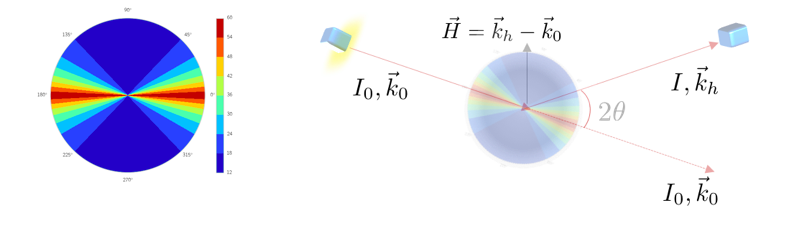
\includegraphics[width=0.9\textwidth]{images/atom_factor.png}
  \caption{ (Слева) фактор рассеяния для атома лантана (La, N = 57), (справа)
  схема расположения векторов для падающей и рассеянной волн}
  \label{ris:atom_factor}
\end{figure}

Приближенное выражение для расчета атомного фактора рассеяния
представляется \cite{International_Tables} в виде выражения:

\begin{equation}
  f_0 = \sum_{i=1}^{4} \cdot a_i e^{ -b_i (\frac{sin \vartheta_B}{\lambda})^2} + C
 \end{equation}
где $a_i$, $b_i$ и $c$ - коэффициенты Кромер-Манна для бездисперсионного канала рассеяния атомами решетки,
ограничением является $0<\frac{sin\vartheta}{\lambda}<2.0 \angstrom ^{-1}$.
 Характерная зависимость структурного фактора от угла рассеяния и длины волны
для атомов входящих в состав кристалла LGT (La, Ga, Ta, O) представлена на рис. \ref{ris:atom_factor_GaLaTa}.

\begin{figure}[H]
  \centering
  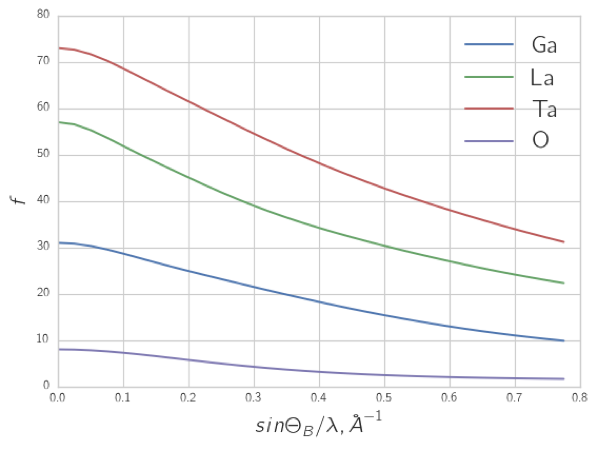
\includegraphics[width=0.6\textwidth]{images/atom_factor_GaLaTa.png}
  \caption{ Атомный фактор рассеяния для атомов: галлия (Ga), лантана (La), тантала (Ta) и  кислорода (O)}
  \label{ris:atom_factor_GaLaTa}
\end{figure}

При расчете интенсивности рассеяния атомом необходимо учитывать факт,
что все электроны связаны между собой, таким образом необходимо записывать
уравнение движение связанного электрона по действием падающего излучения.
Если атом многоэлектронный, то амплитуда рассеянной волны равна сумме амплитуд волн,
рассеянных всеми электронами атома, в результате структурный фактор \cite{iveronova1972}:

\begin{equation}
  f = f_0 + f^{'} + i f^{''}
 \end{equation}
\noindent
где, $f_0$ - атомный фактор рассеяния, рассчитанный без учета сил связи электронов
 с ядром, а $f^{'}$ и $f^{''}$ - дисперсионные поправки \cite{f0f1f12},
 первая из которых учитывает дополнительное рассеяние,
а вторая - дополнительное поглощение вблизи собственных частот колебаний электронов в атоме.

 \begin{figure}[H]
   \centering
   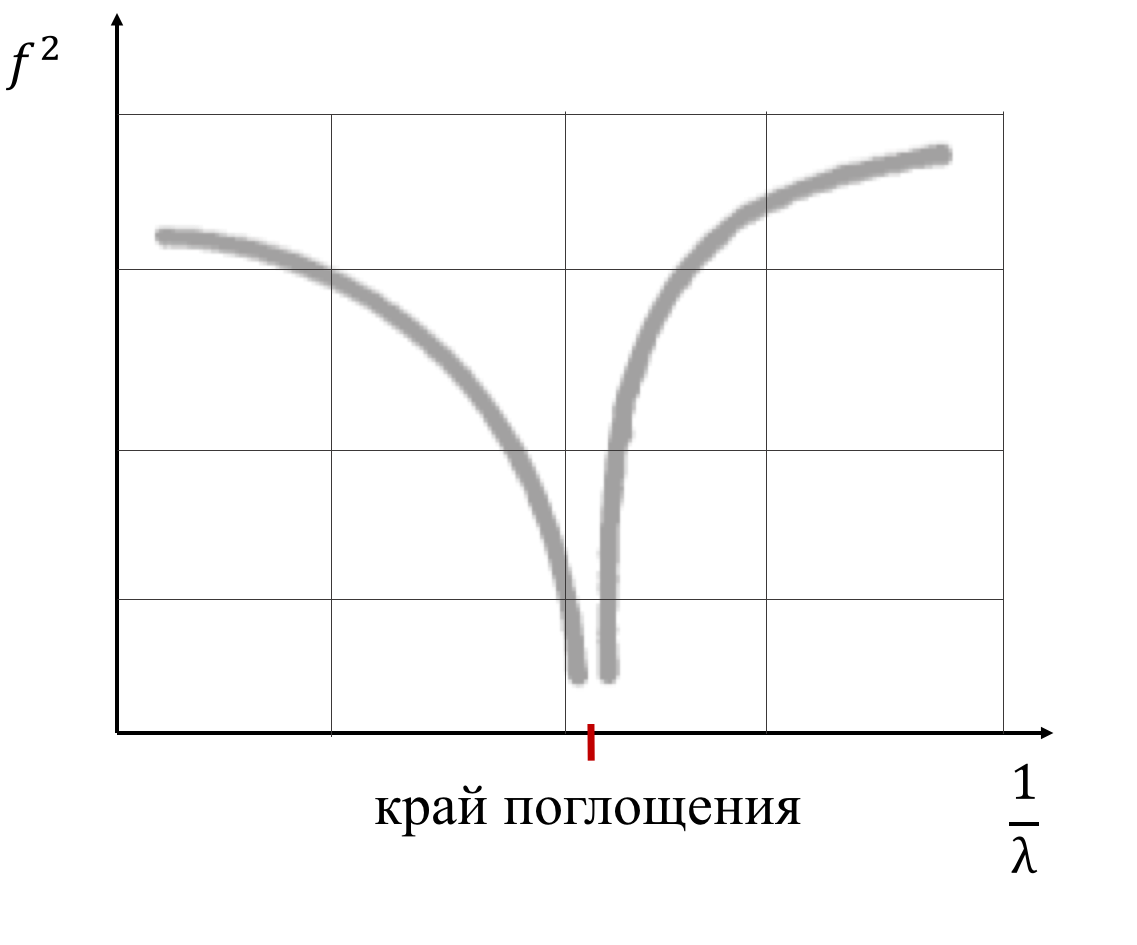
\includegraphics[width=0.4\textwidth]{images/dispers_f.png}
   \caption{ Схематичная зависимость квадрата атомного фактора $f^2 = (f_0 + f^{'})^2 + (f^{''})^2 $ от
   длины волны $\lambda$ вблизи края поглощения}
   \label{ris:dispers_f}
 \end{figure}

Важной особенностью является факт того, что дисперсионные поправки $f^{'}$, $f^{''}$
практически не зависят от длины волны, но зависят от энергии. Так как $f_0$ уменьшается
с ростом угла рассеяния, дисперсионные поправки начинают играть роль при больших углах $\theta$.

\label{sec:structure_factor}
Атомы решетки, взаимодействуя с рентгеновским излучением, рассеивают его.
Если в элементарной ячейке более одного атома, волны от разных атомов,
 интерферируя между собой, вносят вклад в общую картину рассеяния,
 ослабляя или усиливая ее.

 \begin{figure}[H]
   \centering
   \subfloat[]{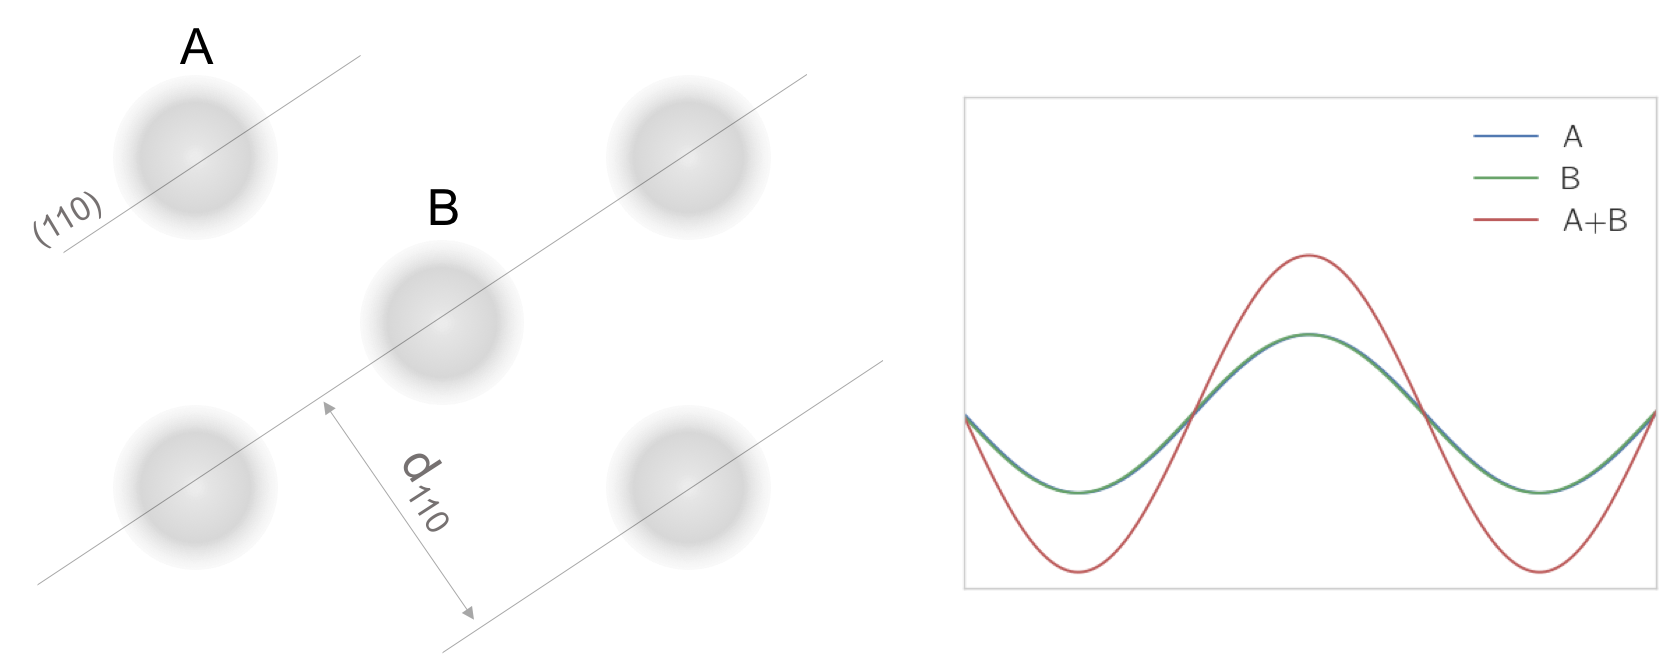
\includegraphics[width=0.45\textwidth]{images/interference_construct.png}}
   \hfill
   \subfloat[]{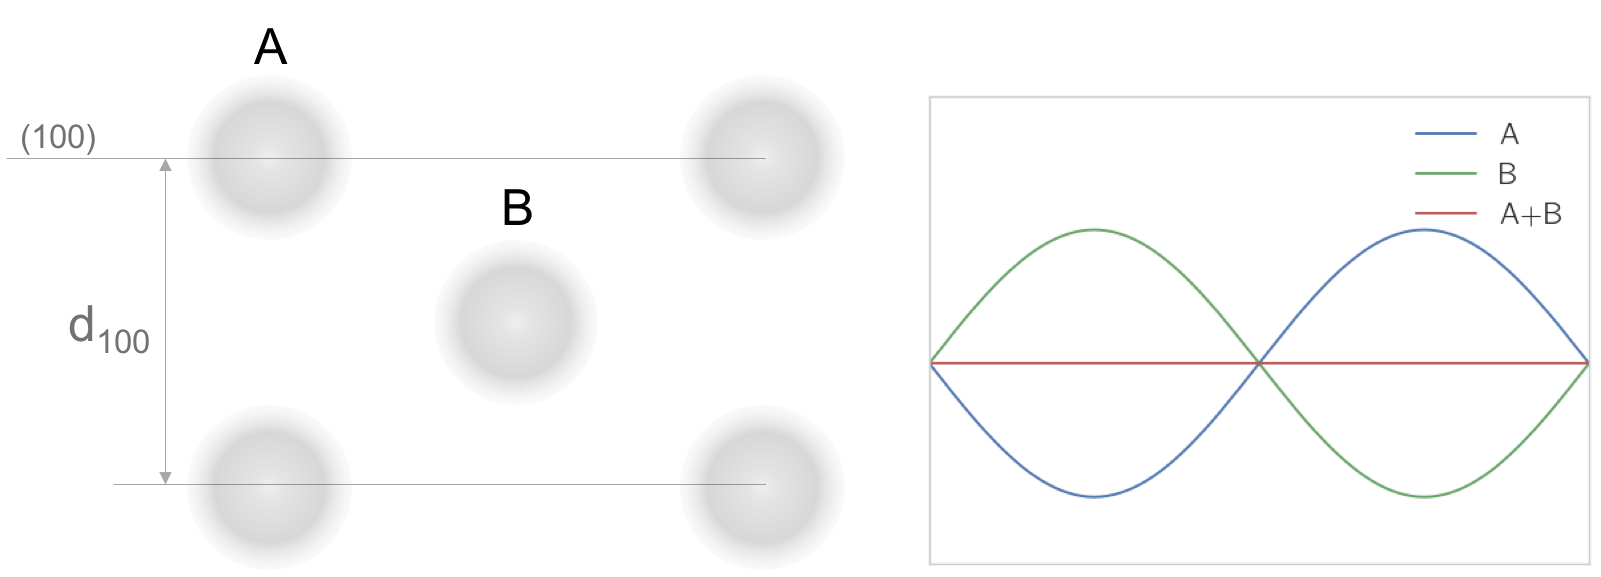
\includegraphics[width=0.45\textwidth]{images/interference_destruct.png}}
   \caption{Примеры интерференции двух волн, отраженных различными системами атомных плоскостей для случая
   конструктивной (a) и деструктивной (b) интерференции}
   \label{ris:interference_by_plate}
 \end{figure}

Рассеяние от набора атомов характеризуется структурным фактором, определяемым векторным
 сложением фаз по всем N атомам элементарной ячейки:

 \begin{equation}
   F = \sum_{n} f_n e^{ i\vec{h}\vec{r}_n} =   \sum_{n} f_n \cdot e^{-i\phi_n},
   \label{eq:F_factor}
  \end{equation}
\noindent
где $\phi_n = 2 \pi (hx_n+ky_n+lz_n)$;  $h, k, l$ - индексы Миллера; $x, y, z$ - относительные координаты
атомов в элементарной ячейке.

В соответсвии с \ref{eq:F_factor} в качестве примера был произведен расчет трехмерной ($hkl$) -
карты струкутрного фактора (рис. \ref{ris:hkl_LGT_SI}).
Цветом изображена величина структурного фактора для разных
 индексов плоскостей отражения для кристаллов LGT и Si.
 В таком представлении просматривается периодичность образования запрещенных
 рефлексов в кубическом кремнии. В кристалле LGT запрещенных (синий цвет)
  индексов для отражения на порядок меньше, связанно это с более низкой
  симметрией кристалла.

  \begin{figure}[h]
    \centering
    \subfloat[]{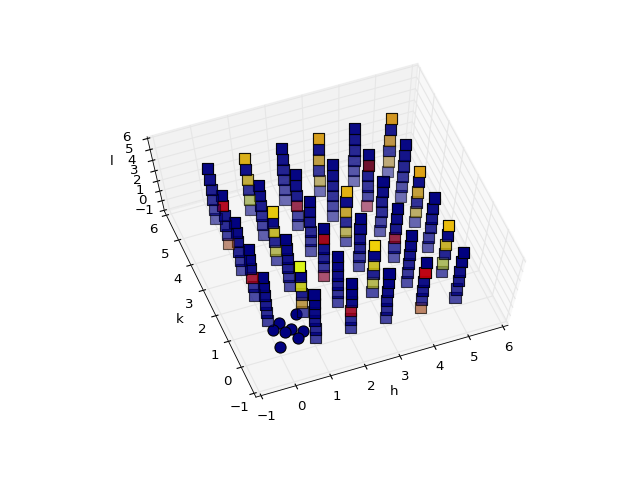
\includegraphics[width=0.5\textwidth]{images/hkl_Si.png} \label{ris:hkl_LGT_SI_a}}
    \hfill
    \subfloat[]{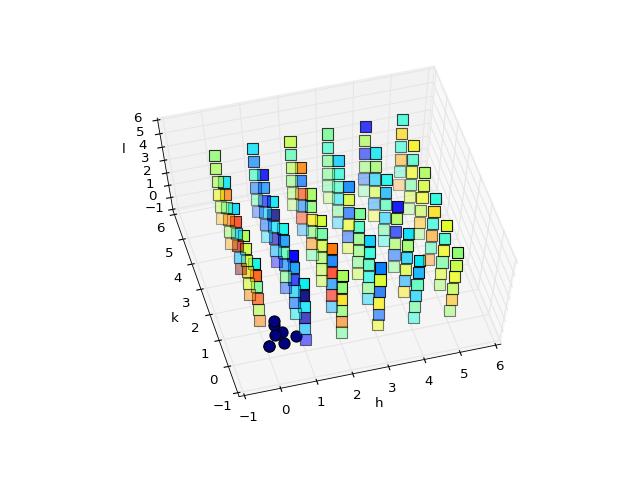
\includegraphics[width=0.5\textwidth]{images/hkl_LGT.png} \label{ris:hkl_LGT_SI_b}}
    \caption{Карта распределения величины структурного фактора
    (цвет соответствует его величине) в координатах индексов Миллера для кристалла Si (a) и LGT (b)}
    \label{ris:hkl_LGT_SI}
  \end{figure}

\subsection{Влияние температуры. Тепловой фактор}

При расчете структурных амплитуд рассеяния необходимо учитывать
тепловые колебания атомов в решетке. Предположим, что атомы колеблется около положения
равновесия независимо друг от друга, тогда это эквивалентно увеличения радиуса атома,
что приводит к более быстрому спаду функции атомного рассеяния с ростом угла рассеяния.
С другой стороны эффективное увеличение радиуса атома, очевидно должно зависеть от
величины среднеквадратичного смещения смещения атома  $<u^2>$ из положения равновесия.
Также для простоты предположим, что период тепловых колебаний атомов намного больше периода
колебаний падающего излучения, тем самым мы можем считать атом неподвижным в момент рассеяния,
т.е. пренебречь эффектом Доплера.

Таким образом структурный фактор необходимо усреднить за время наблюдения по всем возможным отклонениям
\begin{equation}
  F_T = \left\langle \sum_{n} f_n \cdot  e^{-i\vec {h} \cdot (\vec{r_n}+ \vec{u}(t))} \right\rangle =  \sum_{n} f_n \cdot  e^{-i\vec {h} \cdot \vec{r_n}}  \left\langle e^{-i \vec{h} \cdot \vec {u}(t)  } \right\rangle
 \end{equation}

где $\vec{u(t)}$ - отклонение атома во времени, $\vec{r_n}$ - положение атома $n$
в идеальной ячейки, суммирование производится, по всем атомам элементарной ячейки.
$\vec{h}$ - вектор обратной решетки, $|\vec{h}| = 2 \pi / d = $ где $d$ - межплоскостное расстояние.

Разложим экспоненту, содержащую параметр отклонения, в ряд Тейлора:

\begin{equation}
  \left\langle e^{-i \vec{h} \cdot \vec {u}(t)  } \right\rangle = 1 - i  \left\langle \vec{h} \cdot \vec {u} \right\rangle - \frac{1}{2} \left\langle (\vec{h} \cdot \vec {u})^2 \right\rangle+ \ldots
 \end{equation}

 Cреднее значение всех членов нечетной степени будет тождественно равно нулю.
Учитывая,  $ \left\langle (\vec{h} \cdot \vec {u})^2 \right\rangle = q^2 <u^2> <cos(\theta)> = \frac{1}{2}<u^2>h^2$, преобразуем ряд,

\begin{equation}
1 - i  \left\langle \vec{h} \cdot \vec {u} \right\rangle - \frac{1}{2} \left\langle (\vec{h} \cdot \vec {u})^2 \right\rangle+ \ldots = e^{-\frac{1}{2} <u^2> h^2}
 \end{equation}


 \begin{equation}
   F_T =  \sum_{n} f_n \cdot  e^{-i\vec {h} \cdot \vec{r_n}}  e^{-B (\frac{sin\theta_B}{\lambda} )^2 }
  \end{equation}

 где $B = 8 \pi^2 <u^2>$ - температурный коэффициент Дебая - Валлера,
 $(\frac{h}{4\pi})^2=(\frac{sin\vartheta_B}{\lambda})^2$ -
 вектор вектор обратной решетки или вектор рассеяния. Обычно температурный коэффициент
 находится в пределах от $0.20 \angstrom ^2$ до $3.0 \angstrom ^2$.

 Здесь мы ограничились тем, что все колебания в кристалле изотропные
 (изотропное гармоническое приближение), в более общем случае
 температурный коэффициент определяется тенором третьего порядка \cite{Willis1975}.
 В большинстве случаев гармоническое приближение дает адекватное описание, однако при описании
 атомных колебаний в области высоких температур, когда амплитуда колебаний сопоставима с расстоянием
 между соседними атомами, гармоническое приближение некорректно, в этом случае нужно учитывать ангармонические
 поправки \cite{kibalin2015}.
 \begin{equation}
   <u^2> = <u^2_{harm}> (1+2\gamma \alpha T)
  \end{equation}
  где, $\gamma$ - константа Грюнайзена, $\alpha$ - объемный коэффициент теплового расширения, $T$ - температура.
  В случае возрастания температуры кристалла, интенсивность Бреговского рефлекса будет уменьшаться,
  но угловая полуширина отраженной кривой постоянной останется прежней.

 Кроме теплового фактора Дебая-Валлера (динамического), существует и статическая составляющая,
 величина которой в первую очередь зависит от концентрации дефектов в образце,
 такой вклад меньше зависит от температуры, поэтому проведение температурных измерений
 обычно позволяет разделить статический и динамический вклады.


% Разложим второе слагаемое в ряд Тейлора, тогда среднее значение всех членов нечетной степени
% будет тождественно равно нулю. Ограничившись вторым порядком разложения, получим:
%
% \begin{equation}
%   F_T = F \cdot  \left(1 - 4 \pi^2 <u^2> \left( \frac{h}{a} + \frac{k}{b} + \frac{l}{c}\right)^2 \right)
%  \end{equation}

% Мерой смещения атомов при тепловых колебаниях служит
% их среднеквадратичная амплитуда:
% \begin{equation}\label{eq:debay}
%   <u^2> = \frac{9\hbar^2 T}{m k_B \Theta_D^2}
%  \end{equation}
% где $\hbar$ - постоянная Планка, $k_B$ - постоянная Больцмана, $\Theta_D$ - температура Дебая.
% Величина $B$ может варьироваться в диапазоне от $1 \angstrom $ до $ 100\angstrom $.
%
% В случае возрастания температуры кристалла, интенсивность Бреговского рефлекса будет уменьшаться,
% но угловая полуширина отраженной кривой постоянной останется прежней. Удивительным является то, что
% удается получить достаточно узкие кривые отражения от кристалла в котором атомы случайным
% образом смещены относительно равновесных положений, относительное изменение расстояния
% между соседними атомами может составлять до 10$\%$ при комнатной температуре.



\begin{thebibliography}{99}

\bibitem{International_Tables}
  P. J. Brown, A. G. Fox, E. N. Maslen, M. A. O'Keefe and B. T. M. Willis.
  International Tables for Crystallography (2006). Vol. C, ch. 6.1, pp. 554-595
\bibitem{f0f1f12}
J. Coraux, V. Favre-Nicolin, M. G. Proietti et al. // Phys.Rev. B. – 2007. – 75. – 235312

\bibitem{afanasyev1989}
  А. М. Афанасьев, П. А. Александров, Р. М. Имамов. Ренгеновская диагностика
  субмикронных слоев. - Москва: Наука, 1989 г. - 152 с.

\bibitem{pinsker1982}
  З. Г.  Пинскер. Рентгеновская кристаллооптика. - Москва: Наука, 1982 г. - 292 с.

  \bibitem{iveronova1972}
    В. И.  Иверонова, Г. П. Ревкевич. Теория рассеяния ренгеновских лучей. -
    Москва: Издательство московского университета, 1972 г. - 248 с.
\bibitem{Willis1975}
  Willis, B. T. M. Thermal vibrations in crystallography /
  B. T. M. Willis, A. W. Pryor. — Cambridge University Press, 1975. —P. 279.

\bibitem{kibalin2015}
  Ю. А. Кибалин. Диффракционные исследования атомных колебаний в легкосплавных
  металлах, наноструктуррированных внутри пористых сред. [Текст]: автореф. дис. на соиск.
   учен. степ. канд. физ. - мат. наук (01.04.07) /
   Кибалин Юрий Андреевич; НИЦ "Курчатовский институт". – Москва, 2015. – 99 с.

\bibitem{fetisov2007}
  Г. В. Фетисов. Синхротронное излучение. Методы исследования структуры веществ. -
  Москва: ФИЗМАТЛИТ, 2007 г. - 672 с. ISBN 978-5-9221-0805-8.

\bibitem{landau_8_1992}
 Л.Д. Ландау, Е.М. Лифшиц. Теоретическая физика. том 8 –
 Электродинамика сплошных сред, 2-е изд., Москва: Наука, 1992. - 661 с.
 \bibitem{Bushuev_Oreshko_2002}
 В. А. Бушуев, А. П. Орешко. зеркальное отражение рентгеновских лучей в условиях скользящей дифракции.
 Учебное пособие. Москва: МГУ, физический факультет, 2002. - 57 с.
 \bibitem{Tanner_1998}
 D. Keith Bowen, Brain K. Tanner. High Resolution X-Ray Diffractometry and Topography. - United Kingdom: Taylor and Francis, 1998. - 265 p.

\end{thebibliography}
% \cite{Tanner_1998}


\end{document}
